\newcommand{\sg}{\\[2ex]}
\newcommand{\skg}{\\[4.2ex]}
\newcommand{\sgu}{\\[1.2ex]}
\newcommand{\mg}{\\[15.5pt]}
\newcommand{\pim}{$\pi$M1~}
\newcommand{\cpp}{C\nolinebreak\hspace{-.15em}\raisebox{.22ex}{\footnotesize\textbf{+\hspace*{-.1em}+}}\xspace}
\newcommand{\itemfill}{\setlength{\itemsep}{\fill}}
\NewDocumentCommand{\itemspace}{m}{\setlength\itemsep{#1}}
\renewcommand{\quote}[1]{{\color{colthree}\itshape``#1''\par}}
\newcommand{\ra}{$\rightarrow$\xspace}
\newcommand{\bad}[1]{\textcolor{OrangeRed}{#1}}
\NewDocumentCommand{\header}{m O{colthree} O{\normalsize}}{{\color{#2}#3\bfseries#1}}
\NewDocumentCommand{\edu}{O{100} m m m m}{\begin{minipage}{.3\textwidth}\header{#2}[colthree!#1!black]\\[2pt]\footnotesize#3\\#4\\#5\end{minipage}}
\newcommand{\caplab}[2]{\ifthenelse{\equal{#1}{nocap}}{}{\caption{#1}}\ifthenelse{\equal{#2}{nolab}}{}{\label{#2}}}
\newcommand{\pic}[3]{\ifthenelse{\equal{#1}{r}}{\includegraphics[width={#2\textheight}, angle=-90]{#3}}{\includegraphics[height={#2\textheight}]{#3}}}
\NewDocumentCommand{\figw}{m m}{\includegraphics[width=#2\textwidth]{#1}}
\NewDocumentCommand{\figh}{m m}{\includegraphics[height=#2\textheight]{#1}}
% SUBFIG
\DeclareDocumentCommand{\subfig}{O{.49} O{0} O{0} m m O{nocap} O{nolab}}{\begin{subfigure}[t]{#1\textwidth}\vspace*{#2\textheight}\centering\includegraphics[height={#4\textheight}]{#5}\vspace*{#3\textheight}\caplab{#6}{#7}\end{subfigure}}
% SUBFIGS
\DeclareDocumentCommand{\subfigs}{O{fig} m m O{nocap} O{nolab}}{\begin{figure}[ht!]\centering\ifthenelse{\equal{#1}{fig}}{}{#1\hspace*{.05\linewidth}}#2\hspace*{.05\linewidth}#3\caplab{#4}{#5}\end{figure}}
% FIG
\DeclareDocumentCommand{\fig}{O{n} m m O{nocap} O{nolab}}{\begin{figure}[h!]\centering\pic{#1}{#2}{#3}\caplab{#4}{#5}\end{figure}}
% WRAPFIG
\DeclareDocumentCommand{\wrapfig}{O{l} m m O{nocap} O{nolab}}{
	\begin{wrapfigure}{#1}{#2\linewidth}\includegraphics[width={.95\linewidth}]{#3}\caplab{#4}{#5}\end{wrapfigure}}
\DeclareDocumentCommand{\nicetab}{m m O{nocap} O{nolab}}{
	\begin{table}\centering\alternatecolors
	\begin{tabular}{#1}\rowcolor{darkgray!20}\noalign{\hrule height 1.3pt}
	#2
	\noalign{\hrule height 1.3pt}
	\end{tabular}
	\caplab{#3}{#4}
	\end{table}}

\NewDocumentEnvironment{subfigures}{O{nocap} O{nolab} O{!ht}} {\begin{figure}[#3]\centering} {\caplab{#1}{#2}\end{figure}}
%
\NewDocumentEnvironment{tab}{O{} m O{nocap} O{nolab}}
{ \begin{table}[ht!]#1\centering \begin{tabular}{#2} \noalign{\hrule height 1.3pt} }
{ \\\noalign{\hrule height 1.3pt}\end{tabular}\caplab{#3}{#4}\end{table} }
%
\usepackage[framemethod=TikZ]{mdframed}
\usepackage{calc}
\newlength{\myl}
\mdfsetup{roundcorner=6pt, backgroundcolor=gray!5, shadow=true, shadowsize=3pt, linecolor=black!10, leftmargin=0pt, innerrightmargin=0pt, rightmargin=0pt, innerleftmargin=4pt, skipabove=0pt, skipbelow=0pt, nobreak=true}
\usetikzlibrary{shadows}
\renewcommand{\todo}[1]{
	\settowidth{\myl}{TODO: #1}\hspace*{-5pt}
	\begin{minipage}{\the\myl} \begin{mdframed}\small\color{BrickRed}TODO: #1 \end{mdframed}\end{minipage}}
% FRAME W/ BACKGROUND
\newenvironment{bframe}[3] {\usebackgroundtemplate{\includegraphics[width=#3\paperwidth]{#2}}\begin{frame}{#1}} {\end{frame}}
\newenvironment{bframet}[3] {\usebackgroundtemplate{\includegraphics[width=#3\paperwidth]{#2}}\begin{frame}[t]{#1}\vspace*{2ex}} {\end{frame}}
% BLACK/WHITE BOX
\NewDocumentEnvironment{bbox}{m O{1}} { \setbeamercolor{itemize/enumerate body}{fg=white}
\setbeamertemplate{itemize subitem}{
	
\begin{tikzpicture}
		\shade[ball color=gray!70, preaction={fill=black, opacity=.25,transform canvas={xshift=1mm,yshift=-1mm, yscale=0.5}}] (0,0) circle (0.4ex);
	\end{tikzpicture}}
\setbeamertemplate{itemize item}{
	
\begin{tikzpicture}
		\shade[ball color=gray!70, preaction={fill=black, opacity=.25,transform canvas={xshift=1mm,yshift=-1mm, yscale=0.5}}] (0,0) circle (0.6ex);
	\end{tikzpicture}}
	\begin{tcolorbox}[beamer, width=#1\textwidth, no shadow, arc=1mm, opacityback=.5, opacityframe=.5, valign=center, halign=center, left=-1mm, right=1mm, colback=black] \begin{itemize}\addtolength{\itemsep}{#2ex} }
	{ \end{itemize} \end{tcolorbox} }
% GREY BOX
\NewDocumentEnvironment{gbox}{m O{0}} {
	\setbeamertemplate{itemize item}{
		
\begin{tikzpicture}
			\shade[ball color=gray!30, preaction={fill=black, opacity=.25}] (0,0) circle (0.6ex);
		\end{tikzpicture}}
	\begin{tcolorbox}[standard jigsaw, width=#1\textwidth, no shadow, opacityframe=0, arc=1mm, opacityback=.5, valign=center, halign=center, left=-1mm, right=1mm, colback=gray!20] \begin{itemize}\addtolength{\itemsep}{#2ex} }
	{ \end{itemize} \end{tcolorbox} }
% TRANSPARENT BOX
\NewDocumentEnvironment{tbox}{O{.65} O{2}} {
	\setbeamertemplate{itemize subitem}{
		
\begin{tikzpicture}
			\shade[ball color=gray!70, preaction={fill=black, opacity=.25,transform canvas={xshift=1mm,yshift=-1mm, yscale=0.5}}] (0,0) circle (0.4ex);
		\end{tikzpicture}}
	\setbeamertemplate{itemize item}{
		
\begin{tikzpicture}
			\shade[ball color=gray!70, preaction={fill=black, opacity=.25,transform canvas={xshift=-1mm,yshift=-.5mm, yscale=0.5}}] (0,0) circle (0.6ex);
		\end{tikzpicture}}
	\begin{tcolorbox}[standard jigsaw, width=#1\textwidth, no shadow, opacityframe=0, opacityback=0, valign=center, halign=center, left=-1mm, right=1mm] \begin{itemize}\addtolength{\itemsep}{#2ex} }
	{ \end{itemize} \end{tcolorbox}
}
% CONCLUSION
\newenvironment{conclusion}[1][] {\usebackgroundtemplate{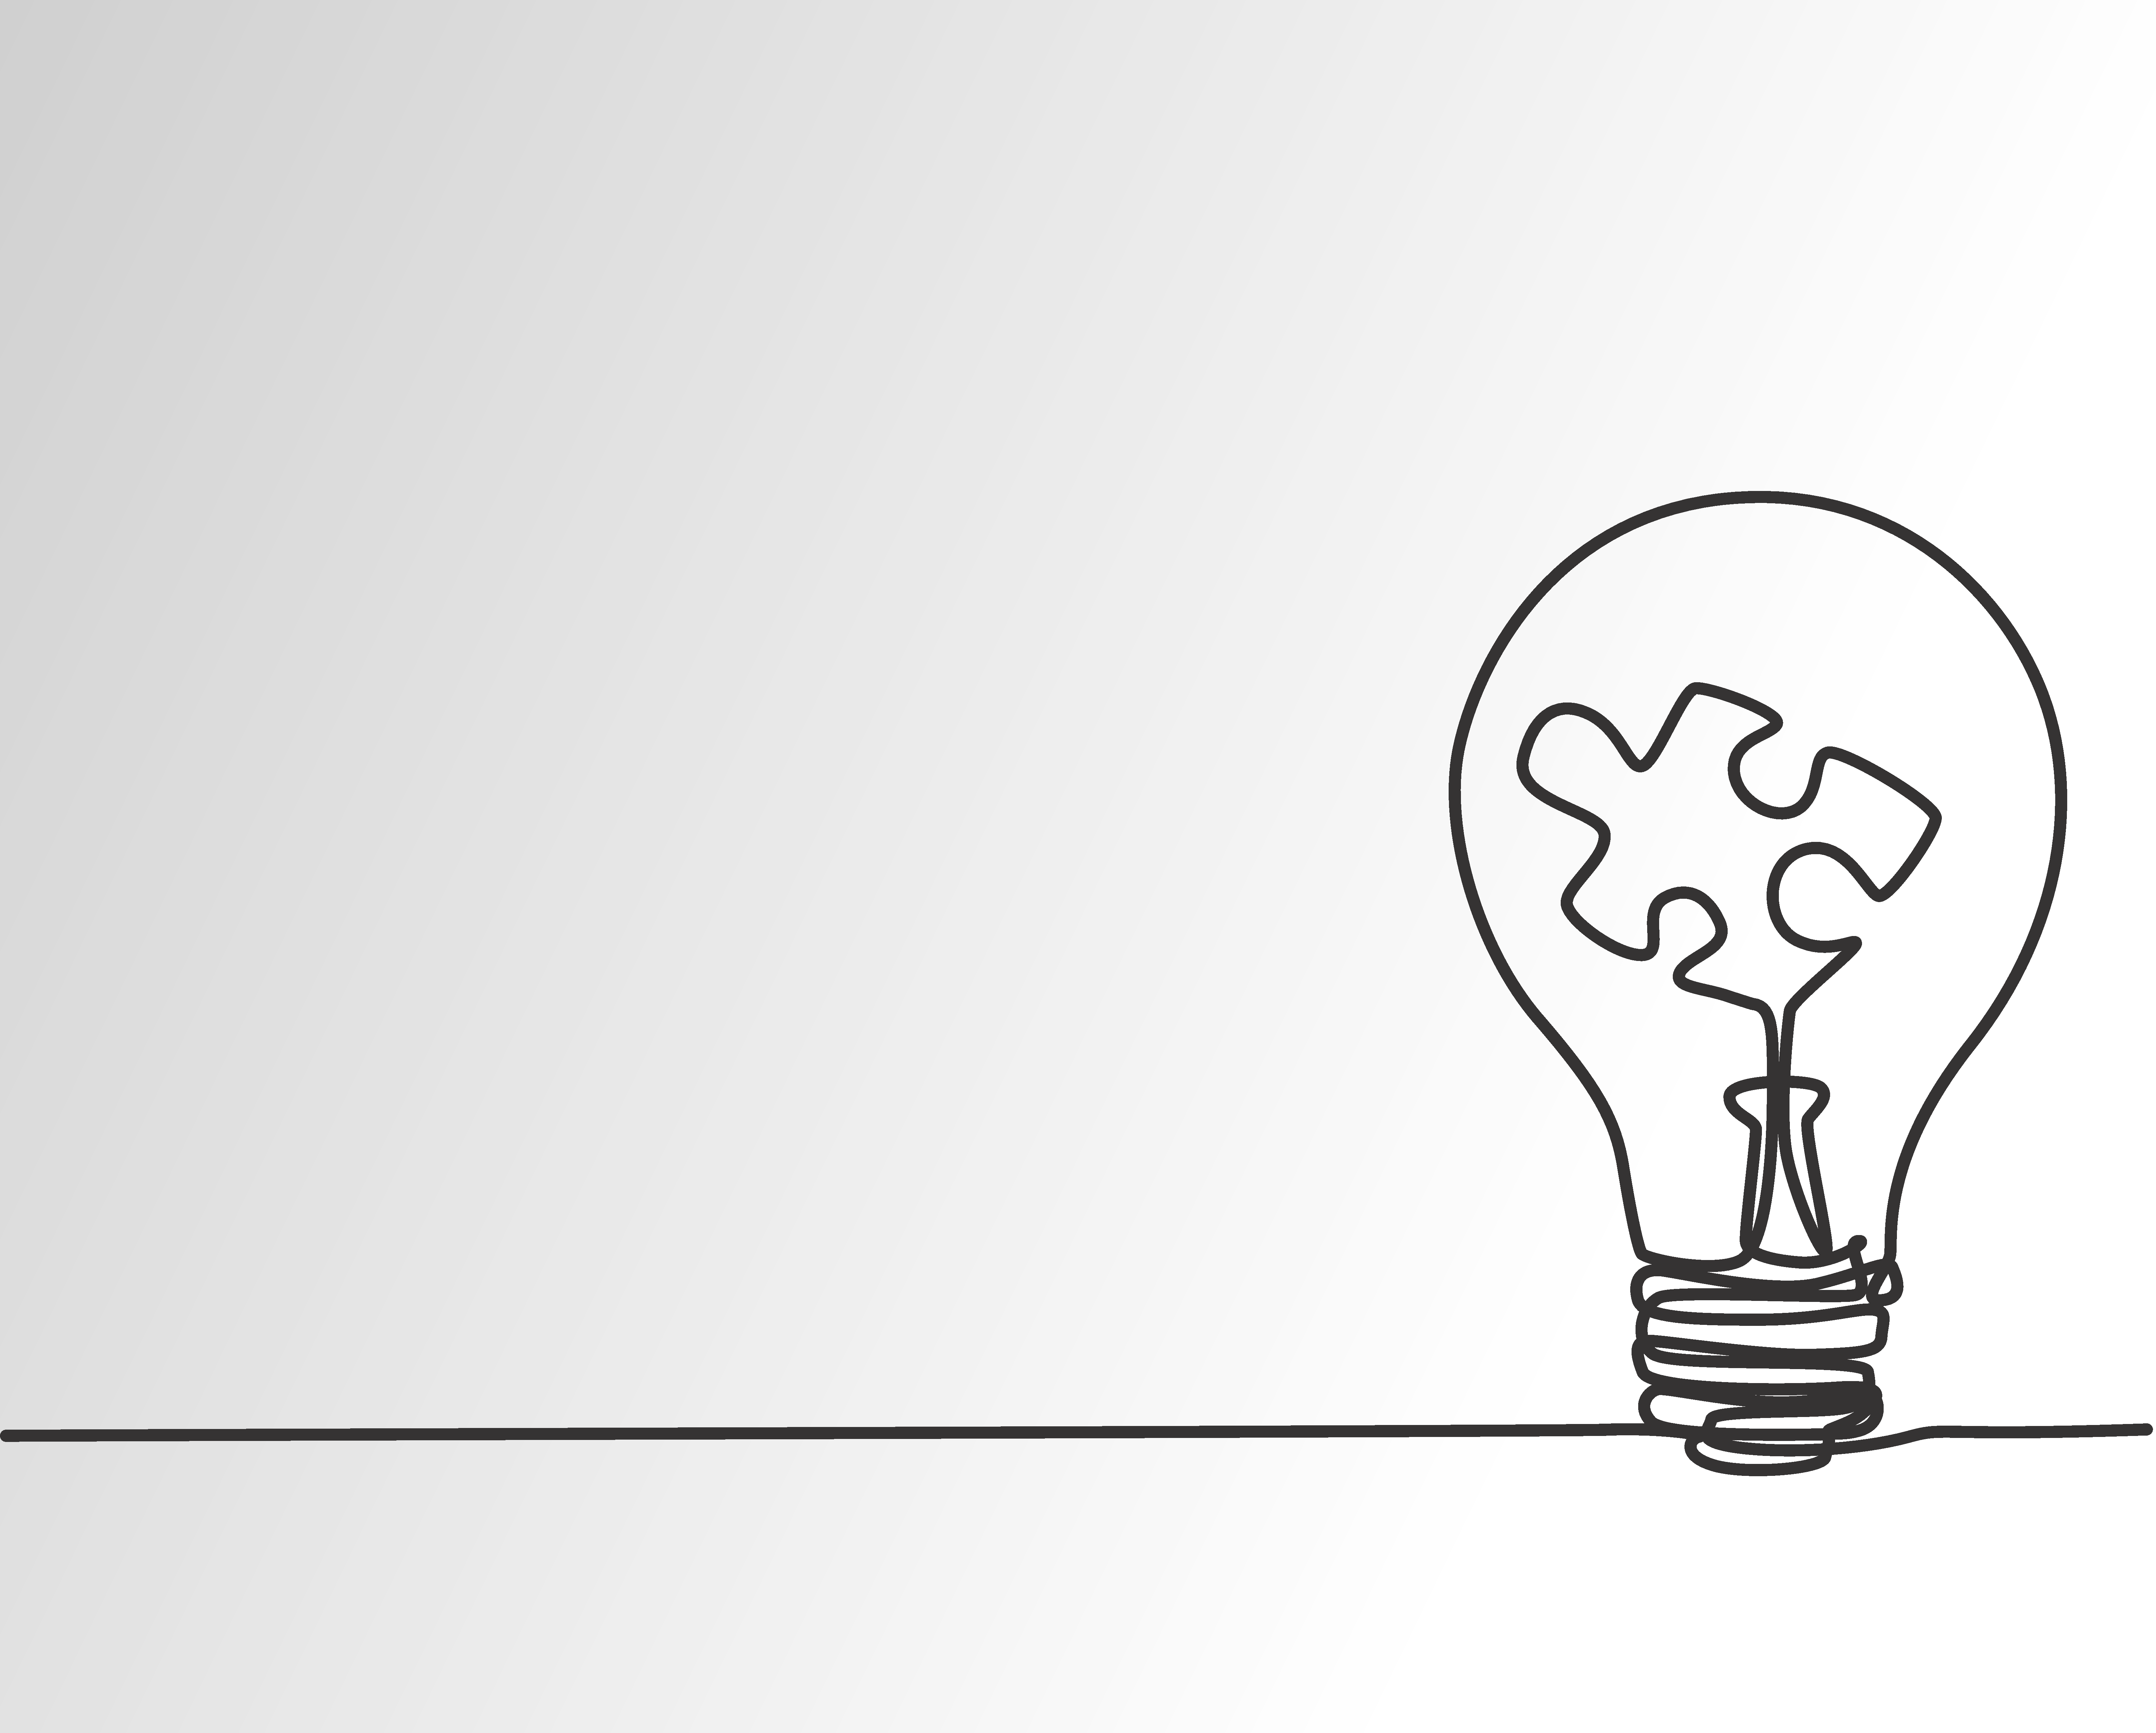
\includegraphics[width=\paperwidth]{figures/main/bulb}}\begin{frame}{Conclusion #1} } { \end{frame} }
% SUMMARY
\newenvironment{summary}[1][] {\begin{frame}{Summary #1} } { \end{frame} }
% PHOTO
\NewDocumentCommand{\roundphoto}{m m O{2pt} O{.5pt} O{darkgray}}{
	\begin{minipage}{#2cm}
		\begin{tikzpicture}
			\path[fill overzoom image={#1}] circle (0.5\linewidth);
			\ifthenelse{\equal{#3}{0}}{}{\draw[line width={#3}, #5] circle (0.5\linewidth)};
			\ifthenelse{\equal{#4}{0}}{}{\draw[white, line width={#4}] circle (0.45\linewidth)};
		\end{tikzpicture}
	\end{minipage}}
% SEPERATION LINE
\NewDocumentCommand{\sepline}{O{white} O{1} O{.01}}{
	\begin{minipage}{#3\textwidth}\centering
		\tikz\draw[#1, line width=#2pt,line cap=round] (0,2)--(0,-2);
	\end{minipage}}
\NewDocumentCommand{\seplinea}{m O{darkgray} O{.5} O{.04}}{
	\begin{minipage}{#4\textwidth}\centering
		\tikz{
			\path[top color=white, bottom color=#2,rounded corners=0.3mm] (+-#3pt, -0.03) rectangle (+#3pt, #1);
			\path[top color=#2, bottom color=white,rounded corners=0.3mm] (+-#3pt, 0.03) rectangle (+#3pt,-#1);}
	\end{minipage}}
% SLIDER
\NewDocumentCommand{\slider}{m O{7ex}}{
	\tikz[baseline=-0.1cm]{
		\coordinate (start) at (0,-0.1cm);
		\coordinate (end) at (#2,0.1cm);
		\coordinate (mark) at ($(start|-0,0)!#1!(end|-0,0)$);
		\fill[rounded corners=0.1cm, draw=gray, bottom color=lightgray, top color=darkgray, middle color=lightgray] (start) rectangle (end);
		\shade[draw=darkgray, rounded corners=0.2mm, ball color=colone] (mark) circle(.15) ; } }
\NewDocumentCommand{\pers}{m m m O{7ex}}{\footnotesize #1 \hfill #2\\\centering\slider{#3}[#4]}
% PROGRESS BAR
\NewDocumentCommand{\pbar}{m O{7ex}}{
	\begin{tikzpicture}[rounded corners=2pt,very thin]
		\coordinate (start) at ( 0,   -.1cm);
		\coordinate (end)   at (#2,    .1cm);
		\coordinate (mark)  at (#1*#2, .1cm);
		\fill[rounded corners=0.1cm, draw=gray, bottom color=lightgray, top color=darkgray, middle color=lightgray] (start) rectangle (end);
		\shade[draw=darkgray,top color=colone, bottom color=black,middle color=colone] 		(start) rectangle (mark);
	\end{tikzpicture}}
\NewDocumentCommand{\motiv}{m m O{7ex}}{\parbox{#3}{\flushleft\footnotesize#1} \pbar{#2}[#3]}
\NewDocumentCommand{\skill}{m m O{7ex}}{\pbar{#2}[#3]\\[-6.5mm]\hspace*{-3mm}\parbox{#3}{\flushleft\includegraphics[height=6mm]{#1}}}
\NewDocumentCommand{\placeobj}{m m m}{
	\begin{tikzpicture}[remember picture,overlay]
		\node[outer sep=0pt,inner sep=0pt,anchor=south west]
		at ([xshift=#1\textwidth,yshift=-#2\textheight] current page.north west) {#3};
	\end{tikzpicture}
}